\section{Buffer Tri-estado \label{sec:s4}}

\begin{center}
	\begin{minipage}{12cm}
		\begin{tcolorbox}[title=Actividad 4]
			Completar el código del buffer tri-estado en el lenguaje de su elección. Compilar y simular. Usar el visor RTL y después el \textit{Chip planner} para ver donde se ubica el buffer. No implementar en la tarjeta.
		\end{tcolorbox}	
	\end{minipage}
\end{center}

La visualización RTL del buffer tri-estado en Verilog se muestra en la \autoref{fig:tristate_buffer_rtl}. Al momento de utilizar la herramienta de \textit{Chip Planner} se observa en la \autoref{fig:tristate_buffer_CP} la implementación del modulo en la periferia del dispositivo. Si se acerca la imagen a este elemento (ver \autoref{fig:tristate_buffer_CPZoom}) se puede ver que el buffer fue implementado por la herramienta en la linea de entradas y salidas debido a que los FPGS's manejan a sus puertos con buffers tri-estados para cambiar su función a entrada o salida. En la \autoref{fig:tristate_buffer_CP_A}, \autoref{fig:tristate_buffer_CP_ENABLE} y \autoref{fig:tristate_buffer_CP_F} se observan los pines A, ENABLE y F del modulo y abriendo el contenido de cada uno, se visualiza en la \autoref{fig:tristate_buffer_CP_A_Inside}, \autoref{fig:tristate_buffer_CP_ENABLE_Inside} y \autoref{fig:tristate_buffer_CP_F_Inside} la ubicación de cada puerto en el buffer. Las simulaciones para el código en Verilog se visualizan en la \autoref{fig:tristate_buffer_WaveBi}.

En los Anexos se localiza la descripción del buffer tri-estado. La implementación es muy sencilla, puesto que solo se hace uso de una estructura \textit{if-else} dentro de una lista sensible. Cabe señalar, que se hace uso del valor ``z'' que significa alta impedancia.

\begin{figure}[ht]
	\centering
	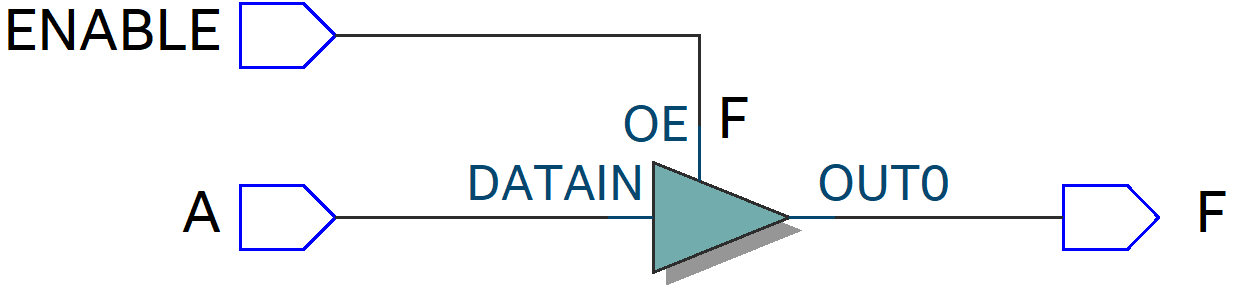
\includegraphics[scale=0.5]{TriState_Buffer_RTL.png}
	\caption{Diagrama RTL del buffer tri-estado. \label{fig:tristate_buffer_rtl}}
\end{figure}

\begin{figure}[ht]
	\centering
	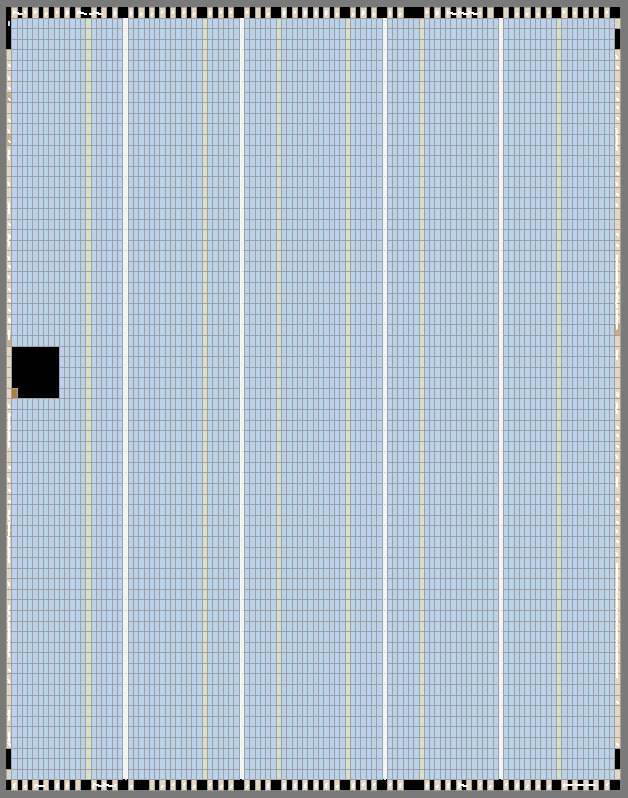
\includegraphics[scale=0.45]{TriState_Buffer_CP.png}
	\caption{Vista de la herramienta de \textit{Chip Planner} del buffer tri-estado. El buffer se observa dentro del circulo rojo. \label{fig:tristate_buffer_CP}}
\end{figure}

\begin{figure}[ht]
	\centering
	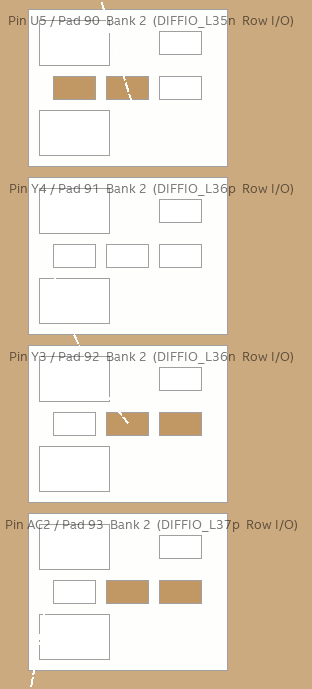
\includegraphics[scale=0.5]{TriState_Buffer_CPZoom.png}
	\caption {Acercamiento al modulo implementado en la línea de entradas y salidas. \label{fig:tristate_buffer_CPZoom}}
\end{figure}

\begin{figure}[ht]
	\centering
	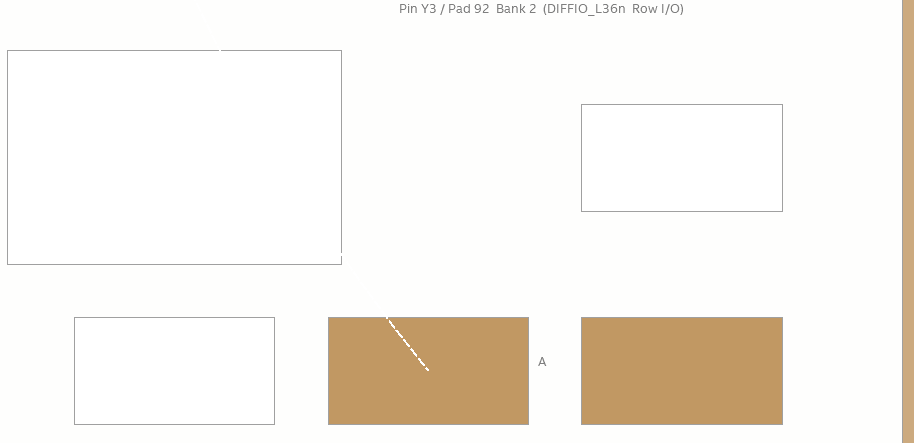
\includegraphics[scale=0.5]{TriState_Buffer_CP_A.png}
	\caption{Vista del pin A. \label{fig:tristate_buffer_CP_A}}
\end{figure}

\begin{figure}[ht]
	\centering
	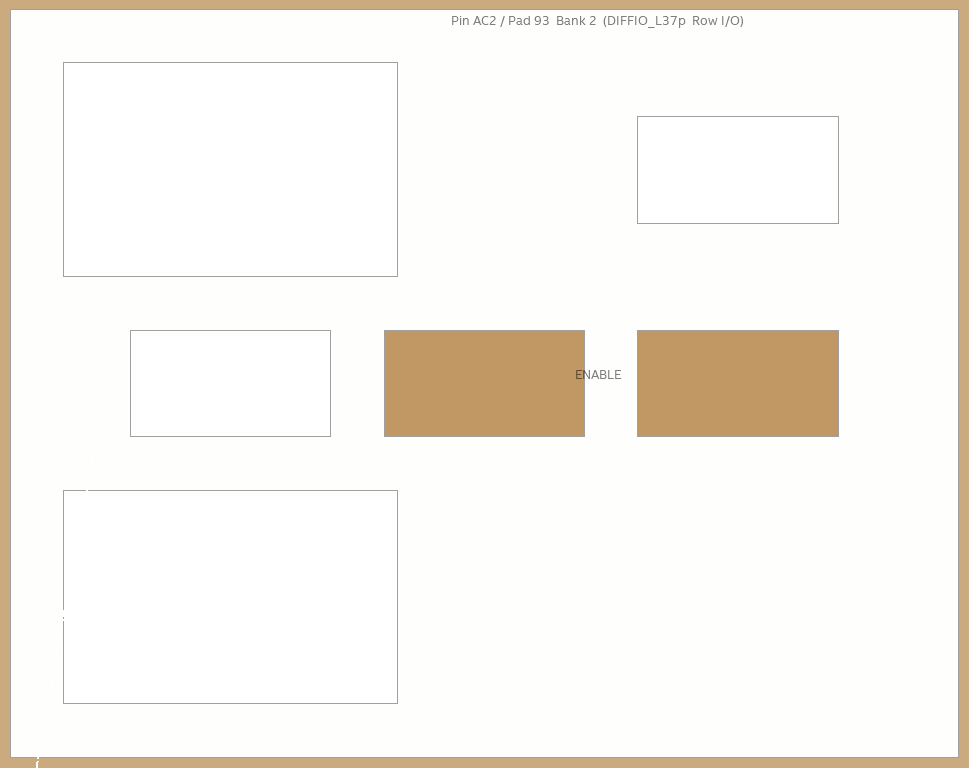
\includegraphics[scale=0.5]{TriState_Buffer_CP_ENABLE.png}
	\caption{Vista del pin ENABLE. \label{fig:tristate_buffer_CP_ENABLE}}
\end{figure}

\begin{figure}[ht]
	\centering
	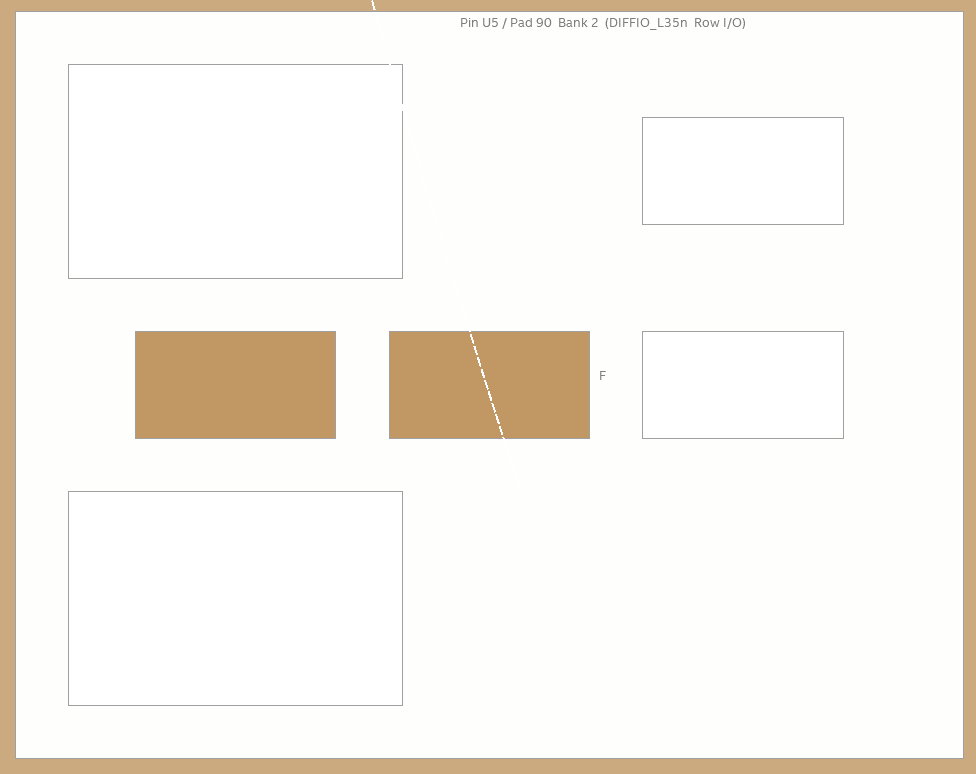
\includegraphics[scale=0.5]{TriState_Buffer_CP_F.png}
	\caption{Vista del pin F. \label{fig:tristate_buffer_CP_F}}
\end{figure}

\begin{figure}[ht]
	\centering
	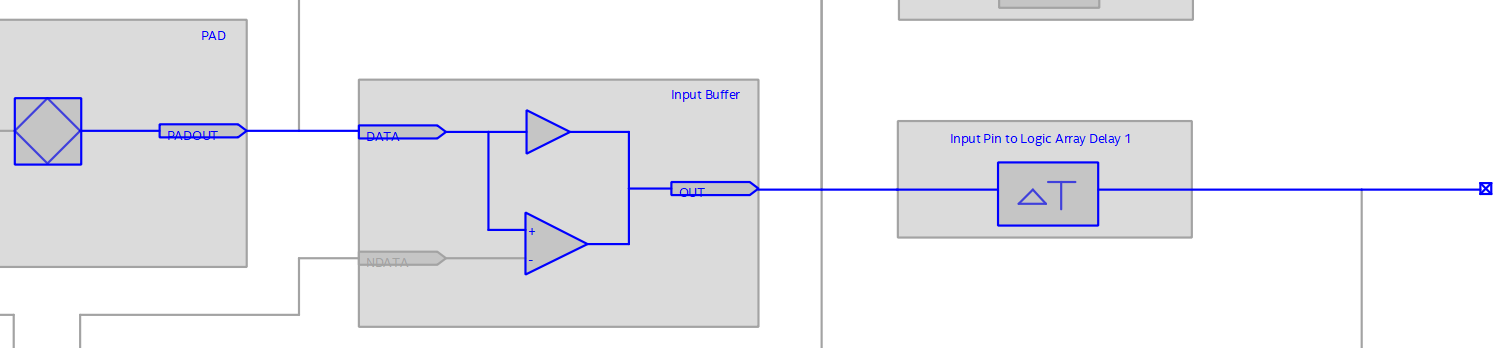
\includegraphics[scale=0.4]{TriState_Buffer_CP_A_Inside.png}
	\caption{Vista del pin A implementado en el buffer. \label{fig:tristate_buffer_CP_A_Inside}}
\end{figure}

\begin{figure}[ht]
	\centering
	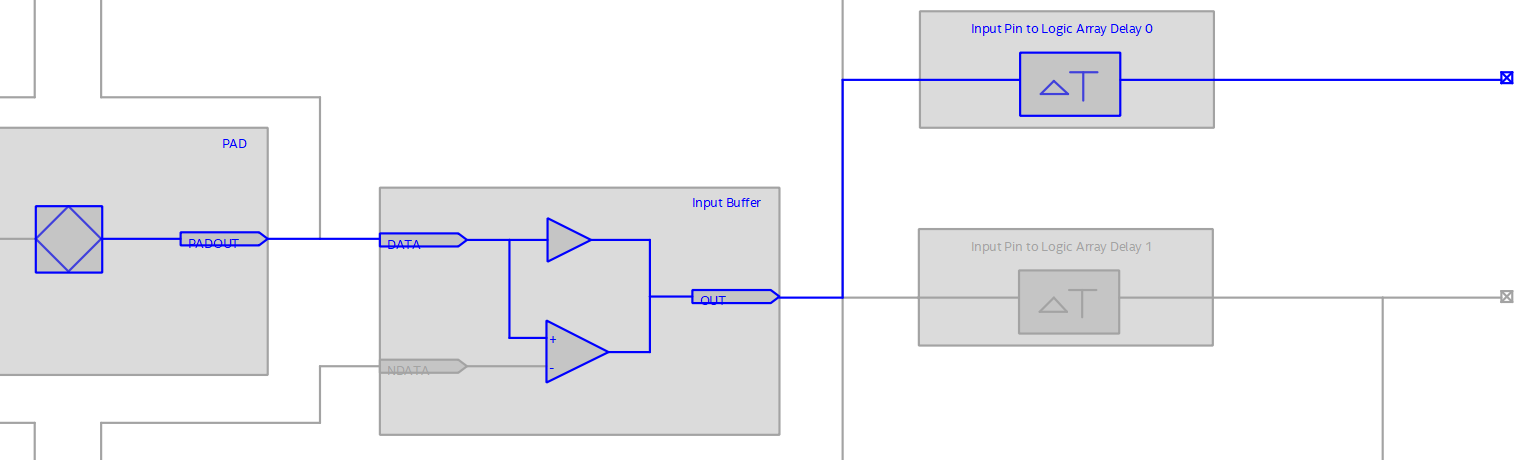
\includegraphics[scale=0.4]{TriState_Buffer_CP_ENABLE_Inside.png}
	\caption{Vista del pin ENABLE implementado en el buffer. \label{fig:tristate_buffer_CP_ENABLE_Inside}}
\end{figure}

\begin{figure}[ht]
	\centering
	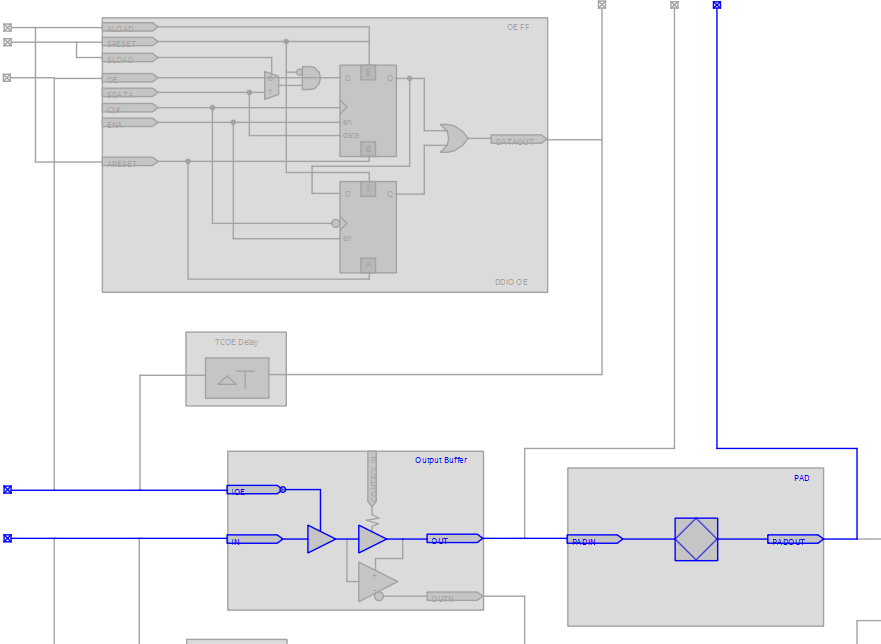
\includegraphics[scale=0.4]{TriState_Buffer_CP_F_Inside.png}
	\caption{Vista del pin F implementado en el buffer. \label{fig:tristate_buffer_CP_F_Inside}}
\end{figure}

\begin{figure}[ht]
	\centering
	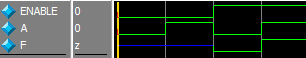
\includegraphics[scale=1.5]{TriState_Buffer_WaveBi.png}
	\caption{Simulación del buffer tri-estado con el visor de formas de onda de ModelSim. \label{fig:tristate_buffer_WaveBi}}
\end{figure}